\chapter{Implementacja}
\thispagestyle{chapterBeginStyle}

\section{Opis komponentów i ich połączeń}
    W programie implementującycm algorytm będący obiektem badań można wyróżnić 3 główne komponenty:
    \begin{itemize}
        \item \textbf{Algorytm} zaimplementowany w języku programowania \textbf{PROLOG}
        \item \textbf{Generowanie grafów} zaimplementowanie w formie modułu w języku programowania \textbf{Python}
        \item \textbf{Warstwa graficzna} (GUI) zaimplementowana w języku programowania \textbf{Python} przy użyciu bibloteki \textbf{Tkinter}
    \end{itemize}
    Naistostniejszą z perspektywy użytkownika jest \textbf{Warstwa graficzna}. Jest to program, którego uruchomienie pozwala na 
    interakcję z utworzonym narzędziem w przyjazny dla użytkownika sposób. Istnieje również możliwość uruchomienia algorytmu z pominięciem 
    warstwy graficznej, o czym można przeczytać w sekcji \ref{CommandLine}.
    Z wyświetlonego menu użytkownik może wybrać przykładowe, wcześniej spreparowane światy, zdefiniować swój stan początkowy oraz cel (w niektórych 
    światach cel jest intuicyjny, więc jego definicja nie jest od użytkownika wymagana) i uruchomić algorytm. Wynikiem działania programu jest 
    plan, który wyświetlony jest w formie tekstowej z opisem na kroki, oraz dwa grafy: graf pełen (zawierający wszystkie składowe opisane 
    w \ref{GRAPHPLANRozdzial}) oraz graf uproszczony, który zawiera jedynie niezbędne stany oraz akcje wymagane do zrozumienia wygenerowanego planu.
    Poniższy schemat klarownie przedstawia relacje między komponentami w trakcie działania programu:
    \begin{figure}[H]
        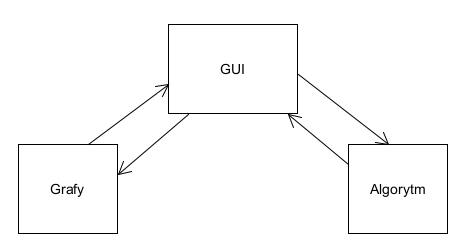
\includegraphics[scale=0.5]{zaleznosci}
        \centering
        \caption{Zależności między komponentami}
    \end{figure}
    Główna jednostką sterującą jest warstwa graficzna. W momencie naciśnięcia przez użytkownika odpowiedniego przycisku generującego rozwiązania, warstwa 
    graficzna zbiera wszystkie niezbędne informacje: w jakim świecie użytkownik pracuje, w jaki sposób zdefiniował warunki początkowe, oraz jakie cele 
    chce on uzyskać. Następnie obrobione informacje przesyłane są do algorytmu, który poza wygenerowaniem planu, do pliku tekstowego wypisuje 
    stany, akcje oraz mutexy dla każdej z warstw.Niestety umieszczanie informacji z każdej warstwy w formie pliku tekstowego 
    znacznie wpływa na czas działania programu, jednakże bez tych informacji wygenerowanie pełnego grafu byłoby niemożliwe. 
    Następnie algorytm przesyła swoją odpowiedź do GUI, który wysyła żadanie wygenerowania grafów do odpowiednich komponentów odpowiedzialnych za ich 
    generowanie. W skład komponentu "Grafy" wchodzą dwie klasy, przy czym każda z nim generuje unikalny graf.

\section{Implementacja algorytmu}
    Algorytm \textbf{GRAPHPLAN} został zaimplementowany w języku programowania PROLOG. Poniższy obrazek przedstawia diagram stanów dla 
    generowania pojedynczego planu.

    //Tutaj rysunek + opis ważniejszych funkcji

\section{Generowanie grafów}
    Moduł generowania grafów utworzony w języku programowania \textbf{python} oraz przy użyciu biblioteki \textbf{graphviz}, zgodnie ze swoją nazwą,
    ma za zadanie wygenerowanie grafów na podstawie otrzymanych informacji od algorytmu. Proces generowania pojedycznego grafu został przedstawiony 
    przy pomocy następującego diagramu stanów:

    //Tutaj rysunek + opis ważniejszych funkcji

\section{Interfejs użytkownika}
    Interfejs użytkownika wykonany w języku \textbf{python} stanowi spoiwo, łącząc w sobie wygenerowany plan przez algorytm oraz wygenerowane grafy przez 
    odpowiedni moduł. Poniższa rycina przedstawia w sposób ogólny diagram stanów w trakcie obsługi programu przez użytkownika:

    //Tutaj rysunek + opis ważniejszych funkcji


\section{Uruchomienie algorytmu z linii komend}
    \label{CommandLine}
    Zalecanym sposobem uruchomienia algorytmu jest wykorzystanie specjalnie przygotowanego programu graficznego, jednakże implementacja zezwala na 
    wykonywanie planów z linii komend. Ów funkcjonalność została wykorzystana między innymi w testach, których opis można znaleźć w ostatnim rozdziale pracy.
    //Jak odpalić z terminala + co należy dodać
